\begin{figure}[h]
    \centering
    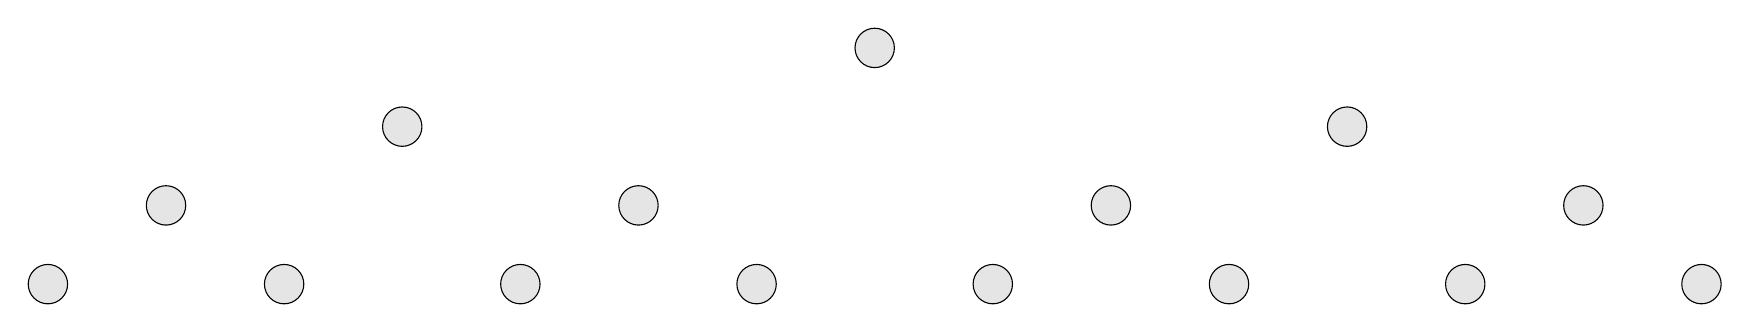
\begin{tikzpicture}[
        vertex/.style={circle, draw, fill=gray!20, minimum size=5mm, inner sep=1pt},
    ]
	\node[vertex] (a_) at (12.0,0) {};
	\node[vertex] (a_0) at (6.0,-1) {};
	\node[vertex] (a_1) at (18.0,-1) {};
	\node[vertex] (a_00) at (3.0,-2) {};
	\node[vertex] (a_01) at (9.0,-2) {};
	\node[vertex] (a_10) at (15.0,-2) {};
	\node[vertex] (a_11) at (21.0,-2) {};
	\node[vertex] (a_000) at (1.5,-3) {};
	\node[vertex] (a_001) at (4.5,-3) {};
	\node[vertex] (a_010) at (7.5,-3) {};
	\node[vertex] (a_011) at (10.5,-3) {};
	\node[vertex] (a_100) at (13.5,-3) {};
	\node[vertex] (a_101) at (16.5,-3) {};
	\node[vertex] (a_110) at (19.5,-3) {};
	\node[vertex] (a_111) at (22.5,-3) {};

    \end{tikzpicture}
    \caption{Cositas.}
    \label{fig:k_tree}
\end{figure}
